
并发程序的开发通常挺难的。有几个因素会使它变得更加困难:例如,编写同时需要正确和高效(换句话说,所有这些都需要)的并发程序要困难得多。对于具有许多互斥对象或无锁程序的复杂程序会更加困难。

正如在上一节的结语中所说的,管理这种复杂性的唯一方法就是对其进行封装,放入定义良好的代码或模块中。只要接口和需求是明确的,这些模块的使用者就不需要知道实现是无锁的还是基于锁的。它确实会影响性能,所以在优化之前,模块对于特定的需求可能不够用,但我们会根据需要进行优化,而且这些优化仅限于特定的模块。

在本章中,我们将重点讨论为并发编程实现数据结构的模块。为什么是数据结构而不是算法?首先,有很多关于并发算法的文献。其次,大多数开发者在处理算法上都有更宽纵的时间:分析代码,相应函数花费了过多的时间,再找到了一种不同的方法来实现算法,并在性能图表上移动到下一个高度。然后,最终会得到一个程序,其中没有一个单独的计算需要花费大量的时间,但您仍然会有它没有达到它应该达到的速度的感觉。我们以前说过,但这需要重复:当没有热代码时,就可能有热数据。

数据结构在并发程序中扮演着更重要的角色,因为它们决定了如何保证算法的可依赖性,以及限制是什么。哪些并发操作可以在相同的数据上安全执行?不同线程看到的数据视图是否一致?如果不知道这些问题的答案,我们就无法编写代码,而答案是由对数据结构的选择而决定的。

与此同时,设计决策,比如接口和模块边界的选择,会对我们编写并发程序时的选择产生重大影响,并发不能作为事后的想法添加到设计中。在设计时,从一开始就必须考虑到并发性,特别是数据的组织。

我们通过定义一些基本的术语和概念开始探索并发数据结构。

\subsubsubsection{6.4.1\hspace{0.2cm}并发数据结构的基础}

使用多线程的并发程序需要线程安全的数据结构。但是什么是线程安全,怎么使数据结构是线程安全的?乍一看,这似乎很简单:如果一个数据结构可以被多个线程同时使用,而没有任何数据竞争(在线程之间共享),那么它就是线程安全的。

然而,这个定义过于简单:

\begin{itemize}
\item 将标准定的很高——例如,没有一个STL容器是线程安全的。
\item 具有非常高的性能开销。
\item 这通常是不必要的,开销也是如此。
\item 除此之外,在许多情况下是完全无用的。
\end{itemize}

我们将逐一解决这些问题。为什么线程安全的数据结构即使在多线程程序中也是不必要的?一种微小的可能性是,用于程序的单线程部分。我们努力最小化这些部分,因为它们对总体运行时的有害影响(还记得Amdahl定律吗?),但是大多数程序都有一些需要单线程处理的事情,我们使这些代码更快的方法是只针对必要的开销。更常见的不需要线程安全的情况是,一个对象仅由一个线程使用,即使是在多线程程序中。这是非常常见的,也是非常可取的:正如我们多次说过的,共享数据是并发程序中效率低下的主要原因,因此我们试图在每个线程上只使用本地对象和数据,独立地完成尽可能多的工作。

但是,我们能确定在多线程程序中使用一个类或一个数据结构是安全的吗?即使每个对象永远不会在线程之间共享。这还真不一定:仅仅因为我们在接口层没有看到任何共享,并不意味着在实现层没有共享。多个对象可以在内部共享相同的数据:静态成员和内存分配器只是其中的一些可能性(我们倾向于认为所有需要内存的对象都通过调用\texttt{malloc()}获得,并且\texttt{malloc()}是线程安全的,而且类也可以实现自己的分配器)。

另一方面,只要没有线程修改对象,在多线程代码中使用许多数据结构是安全的。虽然这似乎是显而易见的,但我们必须再次考虑实现:接口可以是只读的,但实现仍然是可以修改对象。如果你认为这是一种奇异的可能性,请考虑标准的C++共享指针\texttt{std::shared\_ptr}:当复制一个共享指针时,复制的对象不会被修改,至少不会可见(它是通过\texttt{const}引用传递给新指针的构造函数的)。与此同时,知道对象中的引用计数必须增加,这意味着复制的对象已经改变(在此场景中,共享指针是线程安全的,但这不是偶然发生的,也不是免费的,同样也有性能成本)。

我们需要一个更细致的线程安全定义。不幸的是,对于这个普遍的概念,没有通用的标准,但是有几个流行的版本。线程安全的最高级别通常称为\textbf{强线程安全保证},意思是:提供这种保证的对象可以被多个线程并发使用,而不会引起数据竞争或其他未定义的行为(特别是,任何类不变量都会保留)。下一级称为\textbf{弱线程安全保证},只要所有线程都限制为只读访问(调用类的\texttt{const}成员函数),提供这种对象就可以使用多个线程同时访问。其次,任何对对象具有独占访问权的线程都可以对对象执行其他的操作(无论其他线程在同一时间做什么)。不提供任何此类保证的对象,根本不能在多线程程序中使用:即使对象本身不共享,其实现内部的某些内容也很容易被其他线程修改。

本书中,我们将使用强弱线程安全的语言保证。提供强担保的类有时简单地称为\textbf{线程安全}。如果该类只提供弱保证,则称为\textbf{线程兼容}。大多数STL容器都提供了这样的保证:如果容器是一个线程的局部对象,可以以任何有效的方式使用它,但如果容器对象是共享的,只能调用\texttt{const}成员函数。最后,根本不提供任何保证的类被称为\textbf{线程敌对},并且不能使用在多线程程序中。

实践中,我们经常遇到强保证和弱保证的组合:接口的一个子集提供强保证,但其余部分只提供弱保证。

那么,为什么不尝试在设计每个对象时都有强线程安全保证呢?我们已经提到的第一个原因是:会有性能开销,保证通常是不必要的,因为对象不是在线程之间共享的,编写高效程序的关键是不做无用的工作。更有趣的反对意见是我们前面提到的:即使在以需要线程安全的方式共享对象,强线程安全保证可能是无用的。假如需要开发一款玩家招募军队并进行战斗的游戏。军队中所有单位的名称都存储在一个容器中,比如一个字符串列表。另一个容器存储每个单元的当前强度。在战役中,单位总是会被杀死或招募,游戏引擎是多线程的,需要有效地管理庞大的军队。虽然STL容器只提供弱线程安全保证,但假设我们有一个强线程安全容器库。很容易看出这是不够的:添加一个单元需要将它的名称插入到一个容器中,并将它的初始强度插入到另一个容器中,这两个操作本身都是线程安全的。一个线程创建一个新单元并将其插入到第一个容器中。在这个线程还可以添加它的强度值之前,另一个线程看到这个新单位并需要查找它的强度,但是在第二个容器中还没有任何东西。问题在于线程安全保证是在错误的层面上提供的:从应用程序的角度来看,创建一个新单元是一个事务,所有游戏引擎线程都应该能够在添加单元之前或之后查看数据库,但不能在中间状态。例如,可以通过使用互斥锁来实现:它会在单元添加前锁定,只有在两个容器都新之后才会解锁。然而,在这个场景中,我们不关心单个容器提供的线程安全保证,只要这些对象的所有访问都由互斥锁保护。显然,我们需要的是一个单元数据库,它本身提供所需的线程安全保证,例如:通过使用互斥对象。这个数据库可能在内部使用几个容器对象,数据库的实现可能需要或不需要这些容器的任何线程安全保证,但这对数据库的使用者应该是不可见的(拥有线程安全的容器可能会使实现更容易,也可能不会)。

这让我们得出一个非常重要的结论:线程安全始于设计阶段。必须明智地选择程序使用的数据结构和接口,以便它们表示适当的抽象级别,以及发生线程交互级别上的正确事务。

考虑到这一点,本章的其余部分应该从两个方面来看:一方面,将展示如何设计和实现一些基本的线程安全的数据结构,这些数据结构可以用作在程序中需要的更复杂(和更多样化)的构建块。另一方面,还展示了构建线程安全类的基本技术,这些类可用于设计这些更复杂的数据结构。

\subsubsubsection{6.4.2\hspace{0.2cm}计数器和累加器}

最简单的线程安全对象是简单的计数器或累加器,计数器只是计算在线程上可能发生的一些事件。所有线程都可能需要修改计数器或访问当前值,因此存在竞争条件。

弱线程安全保证无法满足我们的要求,这里需要强线程安全保证。从而确保读取没有更改的值总是线程安全的。我们已经看到了实现的可用选项:某种锁、原子操作(当有原子操作时)或无锁CAS循环。

锁的性能因实现的不同而不同,通常首选自旋锁。没有立即访问计数器的线程的等待时间将非常短,因此将线程置于睡眠状态,并在稍后将其唤醒的成本没什么意思。另一方面,由于繁忙等待(轮询自旋锁)而浪费的CPU时间可以忽略不计,很可能只需要几条指令。

原子指令提供了良好的性能,但操作的选择相当有限:在C++中,可以原子地对整数进行加法,但不能做另一些事,例如:对整数进行乘法。这对于简单的计数器来说已经足够了,但是对于累加器来说可能还不够(累加操作可能有多个结果)。但是,如果有一种方法可用,那么它没有原子操作简单。

CAS循环可用于实现累加器,而不考虑我们需要使用的操作。然而,在大多数现代硬件上,性能比自旋锁的性能更好(参见图6.2),但并不是最快的选择。

当使用自旋锁访问单个变量或单个对象时,可以进一步优化自旋锁。我们可以让锁成为保护的对象的唯一引用,而不是通用标志。原子变量是指针,而不是整数,除此之外,锁定机制保持不变。因为\texttt{lock()}函数返回指向计数器的指针,所以是非标准的:

\hspace*{\fill} \\ %插入空行
\noindent
\textbf{01d\_ptrlock\_count.C}
\begin{lstlisting}[style=styleCXX]
template <typename T>
class PtrSpinlock {
	public:
	explicit PtrSpinlock(T* p) : p_(p) {}
	T* lock() {
		while (!(saved_p_ =
		p_.exchange(nullptr, std::memory_order_acquire))) {}
	}
	void unlock() {
		p_.store(saved_p_, std::memory_order_release);
	}
	private:
	std::atomic<T*> p_;
	T* saved_p_ = nullptr;
};
\end{lstlisting}

与之前的自旋锁实现相比,原子变量的含义是“颠倒”:如果原子变量\texttt{p\_}不为空,则该锁可用,否则为空。我们为自旋锁做的所有优化在这里也适用,看起来完全相同,所以我们不打算重复。另外,这个类需要一组删除复制操作(锁是不可复制的)。如果需要将锁转移,并将其释放给另一个对象,则该锁可以移动。如果锁拥有它所指向的对象,析构函数应该删除它(这结合了自旋锁和单类中唯一指针的功能)。

指针自旋锁的第一个优点是,提供了访问保护对象的唯一方式,这就不可能创建竞争条件,并在没有锁的情况下访问共享数据。第二个优点是,锁的性能通常略优于常规自旋锁,自旋锁是否优于原子操作也取决于硬件。相同的基准测试在不同的处理器上会出现非常不同的结果:

%\hspace*{\fill} \\ %插入空行
\begin{center}
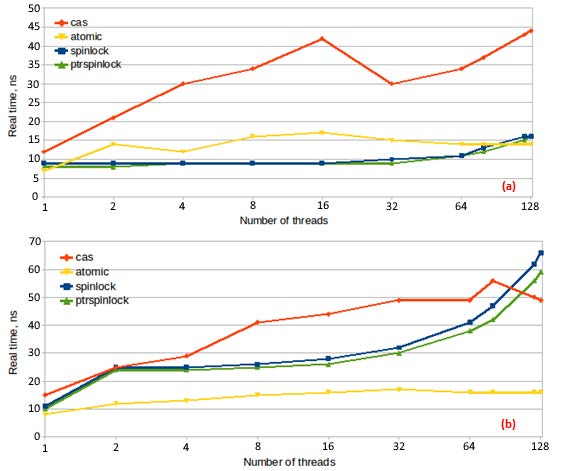
\includegraphics[width=0.9\textwidth]{content/2/chapter6/images/3.jpg}\\
图6.3 - 共享计数增量的性能:不同硬件系统(a)和(b)的常规自旋锁、指针自旋锁、无锁(比较-交换,或CAS)和无等待(原子)
\end{center}

通常,越新的处理器处理锁和繁忙等待的性能越好,而且自旋锁在最新的硬件上提供的性能也越好(图6.3中,系统\textit{b}使用的Intel X86 CPU比系统\textit{a}的CPU晚一代)。

执行一个操作所需的平均时间(或者相反的,吞吐量)是我们在大多数HPC系统中主要关注的指标。然而,这并不是用来衡量并发程序性能的唯一的指标。例如,如果程序在移动设备上运行,那么功耗可能更重要。所有线程使用的CPU总时间根据平均功耗的进行合理的调整。我们用于测量计数器增量平均实时时间的基准测试,同样也可以用来测量CPU时间:

%\hspace*{\fill} \\ %插入空行
\begin{center}
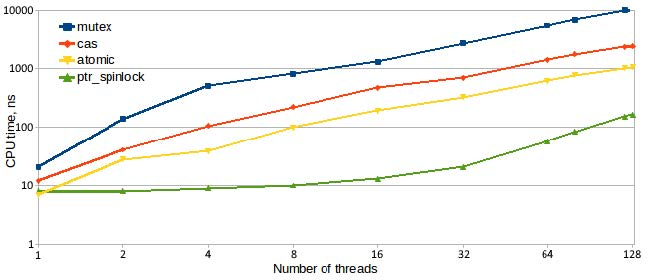
\includegraphics[width=0.9\textwidth]{content/2/chapter6/images/4.jpg}\\
图6.4 - 线程安全的计数器——不同实现使用的平均CPU时间
\end{center}

这里的坏消息是,无论采用哪种实现,多个线程同时访问共享数据的成本都会随着线程数量的增加呈指数增长,至少在有很多线程的情况下是这样的(请注意,图6.4中的y轴比例是对数的)。然而,不同的实现之间的效率差别很大,对于最高效的实现来说,在8个线程之后才会出现指数级的增长。请注意,不同硬件系统的结果也会有所不同,所以必须根据目标平台进行选择,并且只有在完成测试后才能选择。

无论选择何种实现,线程安全的累加器或计数器都不应将其公开,而应将其封装在类中。原因之一是为类的客户端提供稳定的接口,同时保留优化实现的自由度。

第二个原因更微妙,与计数器提供的保证有关。目前为止,我们关注的是计数器本身,确保所有线程都可以对其进行修改和访问,而不存在任何竞争。这是否足够使用,取决于我们如何使用计数器。如果我们想要的只是计算一些事件,而其他东西都不依赖于计数器的值,那么我们只关心值本身是否正确就好。另一方面,如果计数的是数组中的元素数量,那么我们处理的是数据依赖关系。假设有一个大型的预分配数组(或者一个容器,可以在不影响现有元素的情况下增长),所有线程都在计算要插入到这个数组中的新元素。计数器对进行计算的元素进行计数,并将值插入数组,可以由其他线程使用。换句话说,如果一个线程从计数器中读取值N,必须确保数组的前N个元素是安全读取的(这意味着没有其他线程修改它们)。但是数组本身既不是原子的,也不受锁的保护。我们可以通过锁来保护对整个数组的访问,但这可能会降低程序的性能。如果数组中已经有很多元素,任何时候只有一个线程可以读取它们,那么程序就可能是单线程的。另一方面,我们知道从多个线程读取任何常量、不可变数据都是安全的,不需要任何锁。我们只需要知道不可变数据和变化数据之间的边界在哪里,而这正是计数器应该提供的。这里的关键问题是内存可见性:需要保证在计数器的值从N-1更改为N之前,对数组前N个元素的更改对所有线程都可见。

前一章讨论内存模型时已经研究过内存可见性,那时这还是一个理论问题,但现在不是了。从上一章中,我们知道控制可见性的方法是通过限制内存序或使用内存栅栏(同一件事的两种不同的方式)。在多线程程序中,计数和索引的区别在于,索引提供了额外的保证:如果将索引从N-1增加到N的线程在增加索引之前已经完成了数组元素N的初始化,然后其他线程读取索引并获得N(或更大)的值,保证至少有N个元素完全初始化,并且可以安全地读取数组中的元素(假设没有其他线程写入这些元素)。这是一个重要的保证,不要轻易放弃:多个线程正在访问内存中的相同位置(数组元素N)而没有任何锁,其中一个线程正在写入这个位置,访问是安全的,没有数据竞争。若不能使用共享索引来确认这种保证,则需要锁定对数组的所有访问,并且在任何时候只有一个线程能够读取它。相反,我们可以使用这个原子索引类:

\hspace*{\fill} \\ %插入空行
\noindent
\textbf{02\_atomic\_index.C}
\begin{lstlisting}[style=styleCXX]
class AtomicIndex {
	std::atomic<unsigned long> c_;
	public:
	unsigned long incr() noexcept {
		return 1 + c_.fetch_add(1, std::memory_order_release);
	}
	unsigned long get() const noexcept {
		return c_.load(std::memory_order_acquire);
	}
};
\end{lstlisting}

唯一不同的索引在计数是在内存可见性保证,计数不提供:

\begin{lstlisting}[style=styleCXX]
class AtomicCount {
	std::atomic<unsigned long> c_;
	public:
	unsigned long incr() noexcept {
		return 1 + c_.fetch_add(1, std::memory_order_relaxed);
	}
	unsigned long get() const noexcept {
		return c_.load(std::memory_order_relaxed);
	}
};
\end{lstlisting}

The thread safety and memory visibility guarantees should be documented for each of the classes, of course. Whether or not there is a performance difference between the two depends on the hardware. On an X86 CPU, there is none because the hardware instructions for atomic increment and atomic read have the "index-like" memory barriers whether we request them or not. On ARM CPUs, relaxed (or no-barrier) memory operations are noticeably faster. But, regardless of the performance, clarity and intent matter and should not be forgotten: if a programmer uses an index class that explicitly offers the memory order guarantees but does not index anything with it, every reader will wonder what is going on and where is that subtle and hidden place in the code that uses these guarantees. By using the interfaces with the correct set of documented guarantees, you signal to your readers what your intent was when writing this code.

Let us now return to what may be the main "hidden" accomplishment in this section. We learned about thread-safe counters, but along the way, we came up with an algorithm to seemingly violate the first rule of writing multi-threaded code: any time two or more threads access the same memory location and at least one of these threads is writing, all accesses must be locked (or atomic). We did not lock the shared array, we allow arbitrary data in its elements (so it's probably not atomic), and we got away with it! The approach we used to avoid data races turns out to be the cornerstone of almost every data structure designed specifically for concurrency, and we will now take time to better understand and generalize it.

\subsubsubsection{6.4.3\hspace{0.2cm}发布协议}

The general problem we are trying to solve is a very common one in data structure design and, by extension, the development of concurrent programs: one thread is creating new data, and the rest of the program must be able to see this data when it is ready, but not before. The former thread is often called the writer thread or the producer thread. All the other threads are reader or consumer threads.

The most obvious solution is to use a lock and follow the rule of avoiding the data races to the letter. If multiple threads (check) must access the same memory location (check) and at least one thread is writing at this location (exactly one thread in our case – check), then all threads must acquire a lock before accessing this memory location for either reading or writing. The downside of this solution is the performance: long after the producer is done and no more writing happens, all the consumer threads keep locking each other out of reading the data concurrently. Now, read-only access does not require any locking at all, but the problem is, we need to have a guaranteed point in the program such that all the writing happens before this point and all the reading happens after this point. Then we can say that all consumer threads operate in a read-only environment and do not need any locking. The challenge is to guarantee that boundary between reading and writing: remember that, unless we do some sort of synchronization, memory visibility is not guaranteed: just because the writer has finished modifying the memory doesn't mean the reader sees the final state of that memory. The locks include the appropriate memory barriers, as we have seen earlier; they border the critical section and ensure that any operation executed after the critical section will see all the changes to the memory that happened before or during the critical section. But now we want to get the same guarantee without the locks.

The lock-free solution to this problem relies on a very specific protocol for passing information between the producer and the consumer threads:

\begin{itemize}
\item 
The producer thread prepares the data in a memory that is not accessible to other threads. It could be the memory allocated by the producer threads, or it could be pre-allocated memory, but the important point is that the producer is the only thread with a valid reference to this memory, and that valid reference is not shared with other threads (there may be a way for other threads to access this memory, but that would be a bug in the program, similar to indexing an array out of bounds). Since there is only one thread accessing the new data, no synchronization is required. As far as the other threads are concerned, the data simply does not exist.

\item 
All consumer threads must use a single shared pointer for any access to the data, which we call the root pointer, and this pointer is initially null. It remains null while the producer thread is constructing the data. Again, from the point of view of the consumer threads, there is no data at this time. More generally, the "pointer" does not need to be an actual pointer: any kind of handle or reference can be used as long as it gives access to the memory location and can be set to a predetermined invalid value. For example, if all new objects are created in a pre-allocated array, the "pointer" could, in fact, be an index into the array, and the invalid value could be any value greater or equal to the array size.

\item 
The key to the protocol is that the only way for the consumer to access the data is through the root pointer, and this pointer remains null until the producer is ready to reveal, or publish, the data. The act of publishing the data is very simple: the producer must atomically store the correct memory location of the data in the root pointer, and this change must be accompanied by the release memory barrier.

\item 
The consumer thread can, at any time, query the root pointer, again atomically. If the query returns null, then there is no data (as far as the consumer is concerned), and the consumer thread should wait or, ideally, do some other work. If the query returns a non-null value, then the data is ready, and the producer will not change it anymore. The query must be done with the acquire memory barrier, which, in combination with the release barrier on the producer side, guarantees that the new data is visible when the change of the pointer value is observed.
\end{itemize}

This process is sometimes called the publishing protocol because it allows the producer thread to publish information for other threads to consume in a way that guarantees no data races. As we said, the publishing protocol can be implemented using any handle that gives access to the memory as long as this handle can be changed atomically. Pointers are the most common handle, of course, followed by array indices.

The data that is being published can be simple or complex; it doesn't matter. It does not even have to be a single object or a single memory location: the object that the root pointer points to can itself contain pointers to more data. The key elements of the publishing protocol are as follows:

\begin{itemize}
\item
All consumers access a particular set of data through one root pointer. The only way to gain access to the data is to read a non-null value of the root pointer.

\item
The producer can prepare the data any way it wants, but the root pointer remains null: the producer has its own reference to the data that is local to this thread.

\item 
When the producer wants to publish the data, it sets the root pointer to the correct address atomically and with a release barrier. After the data is published, the producer cannot change it (neither can anyone else).

\item 
The consumer threads must read the root pointer atomically and with an acquire barrier. If they read a non-null value, they can read the data accessible through the root pointer.

\end{itemize}

The atomic reads and writes used to implement the publishing protocol should not be, of course, scattered throughout the code. We should implement a publishing pointer class to encapsulate this functionality. In the next section, we will see a simple version of such a class.

\subsubsubsection{6.4.4\hspace{0.2cm}并发编程的智能指针}

The challenge of concurrent (thread-safe) data structures is how to add, remove, and change the data in a way that maintains certain thread safety guarantees. The publishing protocol, which gives us a way to release new data to all threads, is usually the first step in adding new data to any such data structure. Thus, it should come as no surprise that the first class we will learn about is a pointer that encapsulates this protocol.

\hspace*{\fill} \\ %插入空行
\noindent
\textbf{发布指针}

Here is a basic publishing pointer that also includes the functionality of a unique, or owning, pointer (so we can call it a thread-safe unique pointer):

\hspace*{\fill} \\ %插入空行
\noindent
\textbf{03\_owning\_ptr\_mbm.C}
\begin{lstlisting}[style=styleCXX]
template <typename T>
class ts_unique_ptr {
	public:
	ts_unique_ptr() = default;
	explicit ts_unique_ptr(T* p) : p_(p) {}
	ts_unique_ptr(const ts_unique_ptr&) = delete;
	ts_unique_ptr& operator=(const ts_unique_ptr&) = delete;
	~ts_unique_ptr() {
		delete p_.load(std::memory_order_relaxed);
	}
	void publish(T* p) noexcept {
		p_.store(p, std::memory_order_release);
	}
	const T* get() const noexcept {
		return p_.load(std::memory_order_acquire);
	}
	const T& operator*() const noexcept { return *this->get(); }
	ts_unique_ptr& operator=(T* p) noexcept {
		this->publish(p); return *this;
	}
	private:
	std::atomic<T*> p_ { nullptr };
};
\end{lstlisting}

Of course, this is a very bare-bones design; a complete implementation should support a custom deleter, a move constructor and assignment operator, and maybe a few more features, similar to std::unique\_ptr. By the way, the standard does not guarantee that accessing the pointer value stored in a std::unique\_ptr object is atomic or that the necessary memory barriers are used, so the standard unique pointer cannot be used to implement the publishing protocol.

By now, it should be clear to the reader what our thread-safe unique pointer offers: the key functions are publish() and get(), and they implement the publishing protocol. Note that the publish() method does not delete the old data; it is assumed that the producer thread calls publish() only once and only on a null pointer. We could add an assert for that, and it may be a good idea to do so in a debug build, but we are also concerned with the performance. Speaking of performance, a benchmark shows that the single-threaded dereferencing of our publishing pointer takes the same time as that of a raw pointer or of std::unique\_ptr. The benchmark is not complicated:

\begin{lstlisting}[style=styleCXX]
struct A { … arbitrary object for testing … };
ts_unique_ptr<A> p(new A(…));
void BM_ptr_deref(benchmark::State& state) {
	A x;
	for (auto _ : state) {
		benchmark::DoNotOptimize(x = *p);
	}
	state.SetItemsProcessed(state.iterations());
}
BENCHMARK(BM_ptr_deref)->Threads(1)->UseRealTime();
… repeat for desired number of threads …
BENCHMARK_MAIN();
\end{lstlisting}

Running this benchmark gives us an idea of how fast the dereferencing of our lock-free publishing pointer is:

%\hspace*{\fill} \\ %插入空行
\begin{center}
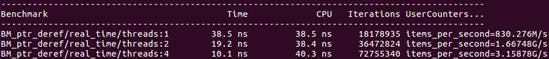
\includegraphics[width=0.9\textwidth]{content/2/chapter6/images/5.jpg}\\
Figure 6.5 – The performance of the publishing pointer (consumer threads)
\end{center}

The result should be compared with dereferencing a raw pointer, which we can also do on multiple threads:

%\hspace*{\fill} \\ %插入空行
\begin{center}
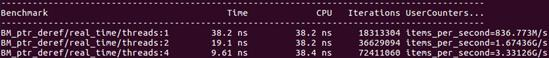
\includegraphics[width=0.9\textwidth]{content/2/chapter6/images/6.jpg}\\
Figure 6.6 – The performance of the raw pointer, for comparison with Figure 6.5
\end{center}

The performance numbers are very close. We can also compare the speed of publishing, but, usually, the consumer side is more important: each object is published only once but then accessed many times.

It is equally important to understand what the publishing pointer does not do. First of all, there is no thread safety in the construction of the pointer. We have assumed that both the producer and the consumer threads share access to the already constructed pointer, which is initialized to null. Who constructed and initialized the pointer? Usually, in any data structure, there is a root pointer through which the entire data structure can be accessed; it was initialized by whatever thread constructed the initial data structure. Then there are pointers that serve as a root for some data element and are themselves contained in another data element. For now, imagine a simple singly linked list where the "next" pointer of every list element is the root for the next element, and the head of the list is the root for the entire list. The thread that produces an element of the list must, among other things, initialize the "next" pointer to null. Then, another producer can add a new element and publish it. Note that this deviates from the general rule that the data, once published, is immutable. This is OK, however, because all changes to the thread-safe unique pointer are atomic. One way or another, it is critical that no thread can access the pointer while it is being constructed (this is a very common restriction, most constructions are not threadsafe, even the question of their thread safety is ill-posed since the object does not exist until it is constructed, so no guarantees can be given).

The next thing our pointer does not do is this: it does not offer any synchronization for multiple producer threads. If two threads attempt to publish their new data elements through the same pointer, the results are undefined, and there is a data race (some consumer threads will see one set of data, and others will see different data). If there is more than one producer thread that operates on a particular data structure, they must use another mechanism for synchronization.

Finally, while our pointer implements a thread-safe publishing protocol, it does nothing to safely "un-publish" and delete the data. It is an owning pointer, so when it is deleted, so is the data it points to. However, any consumer thread can access the data using the value it had acquired earlier, even after the pointer is deleted. The issues of data ownership and lifetime must be handled in some other way. Ideally, we would have a point in the program where the entire data structure or some subset of it is known to be no longer needed; no consumer thread should try to access this data or even retain any pointers to it. At that point, the root pointer and anything accessible through it can be safely deleted. Arranging for such a point in the execution is a different matter entirely; it is often controlled by the overall algorithm.

Sometimes we want a pointer that manages both the creation and the deletion of the data in a thread-safe way. In this case, we need a thread-safe shared pointer.

\hspace*{\fill} \\ %插入空行
\noindent
\textbf{原子共享指针}

If we cannot guarantee that there is a known point in the program where the data can be safely deleted, we have to keep track of how many consumer threads hold valid pointers to the data. If we want to delete this data, we have to wait until there is only one pointer to it in the entire program; then, it is safe to delete the data and the pointer itself (or at least reset it to null). This is a typical job for a shared pointer that does reference counting: it counts how many pointers to the same object are still out there in the program; the data is deleted by the last such pointer.

When talking about thread-safe shared pointers, it is vitally important to understand precisely what guarantees are required from the pointer. The C++ standard shared pointer, std::shared\_ptr, is often referred to as thread-safe. Specifically, it offers the following guarantee: if multiple threads operate on different shared pointers that all point to the same object, then the operations on the reference counter are thread safe even if two threads cause the counter to change at the same time. For example, if one thread is making a copy of its shared pointer while another thread is deleting its shared pointer and the reference count was N before these operations started, the counter will go up to N+1, then back to N (or down first, then up, depending on the actual order of execution) and in the end will have the same value N. The intermediate value could be either N+1 or N-1, but there is no data race, and the behavior is well defined, including the final state. This guarantee implies that the operations on the reference counter are atomic; indeed, the reference counter is an atomic integer and the implementation used fetch\_add() to atomically increment or decrement it.

This guarantee applies as long as no two threads share access to the same shared pointer. How to get each thread its own shared pointer is a separate issue: since all shared pointers pointing to the same object must be created from the very first such pointer, these pointers had to have been passed from one thread to another at some point in time. For simplicity, let us assume, for a moment, that the code that made copies of the shared pointer is protected by a mutex. If two threads access the same shared pointer, then all bets are off. For example, if one thread is trying to copy the shared pointer while another thread is resetting it at the same time, the results are undefined. In particular, the standard shared pointer cannot be used to implement the publishing protocol. However, once the copies of the shared pointer have been distributed to all threads (possibly under lock), the shared ownership is maintained, and the deletion of the object is handled in a thread-safe manner. The object will be deleted once the last shared pointer that points to it is deleted. Note that, since we agreed that each particular shared pointer is never handled by more than one thread, this is completely safe. If, during the execution of the program, the time comes when there is only one shared pointer that owns our object, then there is also only one thread that can access this object. Other threads cannot make copies of this pointer (we don't let two threads share the same pointer object) and don't have any other way to get a pointer to the same object, so the deletion will proceed effectively single-threaded. This is all well and good, but what if we cannot guarantee that two threads won't try to access the same shared pointer? The first example of such access is our publishing protocol: the consumer threads are reading the value of the pointer while the producer thread may be changing it. We need the operations on the shared pointer itself to be atomic. In C++20, we can do just that: it lets us write std::atomic<std::shared\_ptr<T>>. Note that the early proposals featured a new class, std::atomic\_shared\_ptr<T>, instead. In the end, this is not the path that was chosen.

If you do not have a C++20-compliant compiler and the corresponding standard library or cannot use C++20 in your code, you can still do atomic operations on std::shared\_ptr, but you must do so explicitly. In order to publish the object using the pointer p\_ that is shared between all threads, the producer thread must do this:

\begin{lstlisting}[style=styleCXX]
std::shared_ptr<T> p_;
T* data = new T;
… finish initializing the data …
std::atomic_store_explicit(
	&p_, std::shared_ptr<T>(data), std::memory_order_release);
\end{lstlisting}

On the other hand, to acquire the pointer, the consumer thread must do this:

\begin{lstlisting}[style=styleCXX]
std::shared_ptr<T> p_;
const T* data = std::atomic_load_explicit(
	&p_, std::memory_order_acquire).get();
\end{lstlisting}

The major downside of this approach, compared to the C++20 atomic shared pointer, is that there is no protection against accidental non-atomic access. It is up to the programmer to remember to always use atomic functions to operate on the shared pointer.

It should be noted that, while convenient, std::shared\_ptr is not a particularly efficient pointer, and the atomic accesses make it even slower. We can compare the speed of publishing an object using the thread-safe publishing pointer from the last section versus the shared pointer with explicit atomic accesses:

%\hspace*{\fill} \\ %插入空行
\begin{center}
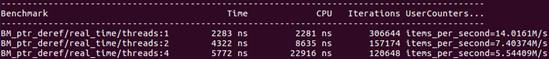
\includegraphics[width=0.9\textwidth]{content/2/chapter6/images/7.jpg}\\
Figure 6.7 – The performance of the atomic shared publishing pointer (consumer threads)
\end{center}

Again, the numbers should be compared with those from Figure 6.5: the publishing pointer is 60 times faster on one thread, and the advantage increases with the number of threads. Of course, the whole point of the shared pointer is that it provides shared resource ownership, so naturally, it takes more time to do more work. The point of the comparison is to show the cost of this shared ownership: if you can avoid it, your program will be much more efficient.

Even if you need shared ownership (and there are some concurrent data structures that are really hard to design without it), usually, you can do much better if you design your own reference-counted pointer with limited functionality and optimal implementation. One very common approach is to use intrusive reference counting. An intrusive shared pointer stores its reference count in the object it points to. When designed for a specific object, such as a list node in our particular data structure, the object is designed with the shared ownership in mind and contains a reference counter. Otherwise, we can use a wrapper class for almost any type and augment it with a reference counter:

\hspace*{\fill} \\ %插入空行
\noindent
\textbf{04\_intr\_shared\_ptr\_mbm.C}
\begin{lstlisting}[style=styleCXX]
template <typename T> struct Wrapper {
	T object;
	Wrapper(… arguments …) : object(…) {}
	~Wrapper() = default;
	Wrapper (const Wrapper&) = delete;
	Wrapper& operator=(const Wrapper&) = delete;
	std::atomic<size_t> ref_cnt_ = 0;
	void AddRef() {
		ref_cnt_.fetch_add(1, std::memory_order_acq_rel);
	}
	bool DelRef() { return
		ref_cnt_.fetch_sub(1, std::memory_order_acq_rel) == 1;
	}
};
\end{lstlisting}

When decrementing the reference count, it is important to know when it reaches 0 (or was 1 before decrementing): the shared pointer must then delete the object.

The implementation of even the simplest atomic shared pointer is quite lengthy; a very rudimentary example can be found in the sample code for this chapter. Again, this example contains only the bare minimum necessary for the pointer to correctly perform several tasks such as publishing an object and accessing the same pointer concurrently by multiple threads. The aim of the example is to make it easier to understand the essential elements of implementing such pointer (and even then, the code is several pages long).

In addition to using an intrusive reference counter, an application-specific shared pointer can forgo other features of std::shared\_ptr. For example, many applications do not require a weak pointer, but there is an overhead for supporting it even if it's never used. A minimalistic reference-counted pointer can be several times more efficient than the standard one:

%\hspace*{\fill} \\ %插入空行
\begin{center}
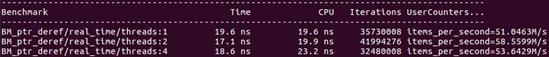
\includegraphics[width=0.9\textwidth]{content/2/chapter6/images/8.jpg}\\
Figure 6.8 – The performance of a custom atomic shared publishing pointer (consumer threads)
\end{center}

It is similarly more efficient for assignment and reassignment of the pointer, atomic exchange of two pointers, and other atomic operations on the pointer. Even this shared pointer is still much less efficient than a unique pointer, so again, if you can manage the data ownership explicitly, without reference-counting, do so.

We now have the two key building blocks of almost any data structure: we can add new data and publish it (reveal it to other threads), and we can track the ownership, even across threads (although it comes at a price).




















